\documentclass{article}
\usepackage{amsmath}
\usepackage{amsfonts}
\usepackage{amssymb}
\usepackage{geometry}
\usepackage{graphicx}
\usepackage{tikz}
\usepackage{listofitems} % for \readlist to create arrays
\tikzstyle{mynode}=[thick,draw=blue,fill=blue!20,circle,minimum size=15]
\geometry{margin=1in}

\title{Analyzing Neural Network Input Spaces through Network Inversion}
\author{Atul Krishnan} 

\begin{document}

\maketitle 





\begin{abstract}
Neural networks are often criticized for their lack of interpretability, earning the nickname "black boxes." This lack of transparency poses significant challenges in practical contexts such as AI safety, where understanding how a model arrives at decisions is crucial for preventing harmful outcomes, and debugging, where identifying the source of errors is essential. This paper introduces a framework for systematically inverting neural networks to reconstruct the input space corresponding to a given output. By leveraging linear algebra and function analysis, this approach identifies and explores the free variables introduced due to differences in layer sizes. These free variables provide insights into the degrees of freedom within the network, enabling a deeper understanding of its behavior and flexibility in generating outputs. Through backward propagation and sampling, the methodology reveals the multidimensional input manifolds associated with specific outputs, offering insights into network behavior, decision boundaries, and potential biases. Initial implementations on small-scale networks validate the feasibility of this approach, with ongoing work focused on scaling to larger architectures.
\end{abstract}



\subsection*{Neural Network Inversion}
Neural network inversion aims to determine the input space corresponding to a given output by propagating backward through the network. The process involves identifying and managing the free variables resulting from layer size mismatches and solving the resulting systems of equations.

\subsubsection*{Forward and Inverse Propagation}

1. \textbf{Forward Propagation Equations}:
\[
wx + b = z, \quad \sigma(z) = a
\]
Forward propagation calculates the output of each layer based on the input, weights, biases, and activation functions. The diagram below illustrates a simple feedforward network:

\begin{center}
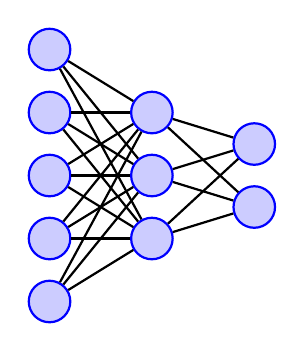
\begin{tikzpicture}[x=1.3cm,y=0.8cm]
  \readlist\Nnod{5,3,2} % number of nodes per layer
  \foreachitem \N \in \Nnod{ % loop over layers
    \foreach \i [evaluate={\x=\Ncnt; \y=\N/2-\i+0.5; \prev=int(\Ncnt-1);}] in {1,...,\N}{ % loop over nodes
      \node[mynode] (N\Ncnt-\i) at (\x,\y) {};
      \ifnum\Ncnt>1 % connect to previous layer
        \foreach \j in {1,...,\Nnod[\prev]}{
          \draw[thick] (N\prev-\j) -- (N\Ncnt-\i);
        }
      \fi
    }
  }
\end{tikzpicture}
\end{center}

2. \textbf{Inverse Propagation Equations}:
\[
 \sigma^{-1}(a) = z, \quad w^{-1} \cdot z  - b = x
\]
Inverse propagation reverses the transformations applied during forward propagation. For each layer, the activation function is inverted, and the weights and biases are used to reconstruct the inputs. Free variables emerge when layer sizes differ, as not all inputs can be uniquely determined by the output. These free variables provide a measure of the network's flexibility, indicating how it balances constraints across layers to produce outputs.

\subsubsection*{Computational Challenges and Limitations}
Inverse propagation introduces several computational challenges:

\textbf{Non-uniqueness of solutions}: Due to free variables introduced by layer size mismatches, multiple input configurations can result in the same output. Sampling these free variables systematically is computationally intensive, especially for deep networks.

\textbf{Non-linear Activation Functions}: The inversion of non-linear activation functions (e.g., sigmoid, ReLU) can lead to numerical instability, especially when dealing with very small or very large outputs.

\textbf{Matrix Inversions}: For layers with high-dimensional weights, inverting matrices becomes computationally expensive, both in terms of time and memory.

\textbf{Error Propagation}: Errors introduced at one layer can amplify as the inversion propagates through subsequent layers, leading to inaccuracies in reconstructed inputs.

Addressing these challenges requires careful optimization of sampling strategies, regularization techniques to stabilize inversions, and efficient numerical methods for handling large-scale matrix operations.

\begin{center}
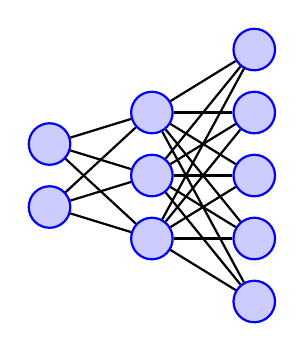
\begin{tikzpicture}[x=1.3cm,y=0.8cm]
  \readlist\Nnod{2,3,5} % number of nodes per layer
  \foreachitem \N \in \Nnod{
    \foreach \i [evaluate={\x=\Ncnt; \y=\N/2-\i+0.5; \prev=int(\Ncnt-1);}] in {1,...,\N}{
      \node[mynode] (N\Ncnt-\i) at (\x,\y) {};
      \ifnum\Ncnt>1
        \foreach \j in {1,...,\Nnod[\prev]}{
          \draw[thick] (N\prev-\j) -- (N\Ncnt-\i);
        }
      \fi
    }
  }
\end{tikzpicture}
\end{center}

\subsubsection*{Matrix Representation and Free Variables}

Consider a simple case with 3 input neurons feeding into 2 hidden neurons:
\[
\begin{bmatrix}
w_{11} & w_{12} & w_{13} \\
w_{21} & w_{22} & w_{23}
\end{bmatrix}
\begin{bmatrix}
x_1 \\
x_2 \\
x_3
\end{bmatrix}
=
\begin{bmatrix}
z_1 \\
z_2
\end{bmatrix}
\]

Here, the mismatch in layer sizes introduces one free variable, which must be sampled during inversion. For example, sampling 100 values for the free variable allows us to explore the full input space associated with the output \(\begin{bmatrix}z_1 \\ z_2\end{bmatrix}\). The sampled values reveal how the network resolves degrees of freedom at each layer.

\subsection*{Simplifying the Linear System}

To reduce the system, eliminate variables systematically. Start with:
\[
\begin{bmatrix}
w_{11} &w_{12} & w_{13} & z_1 \\
w_{21} & w_{22} & w_{23} & z_2
\end{bmatrix}
\]

Eliminate the first column in the second row:
\[
R_2 - \frac{w_{21}}{w_{11}} R_1 \Rightarrow R_2, \quad \frac{w_{21}}{w_{11}} = k
\]

The reduced matrix becomes:
\[
\begin{bmatrix}
w_{11} &w_{12} & w_{13} & z_1 \\
0 & w_{22} - kw_{12} & w_{23} - kw_{13} & z_2 - k z_1
\end{bmatrix}
\]

From here, we can derive equations for \(x_1\) and \(x_2\) by treating \(x_3\) as a free variable.

\subsection*{Representation of Layer \(N-1\)}

For a general case:

1. \textbf{First Equation}:
\[
x_1 = \frac{z_1 - w_{13} x_3 - \left( \frac{(z_2 - k_2)-(w_{23} - kw_{13})}{w_{22} - kw_{12}} \right) x_3}{w_{11}}
\]

2. \textbf{Second Equation}:
\[
x_2 = \frac{(z_2 - k_2)-(w_{23} - kw_{13})}{w_{22} - kw_{12}}
\]

\subsection*{Exploration of Input Spaces}

To interpret neural networks effectively, exploring the input space corresponding to a given output is crucial. Free variables are systematically sampled to reconstruct these spaces. The process involves:

1. Identifying free variables layer by layer.
2. Sampling values for free variables (e.g., 100 samples per variable).
3. Propagating backward using inverse transformations.
4. Visualizing the reconstructed input space as a multidimensional manifold.

\begin{figure}[h]
\centering
\includegraphics[width=0.8\textwidth]{InputVisulization.png}
\caption{Example of input space reconstruction holding \(N-2\) free variables constant. The manifold shows the variety of valid input configurations for a specific output. For instance, when a network output aligns with \([0.8, 0.2]\), this visualization highlights the range of inputs (e.g., specific features or conditions) that lead to this outcome.}
\end{figure}

\subsection*{Applications}

This framework has the following applications:

- \textbf{Model Interpretation:} Understanding input-output relationships.
- \textbf{Debugging:} Identifying sensitivities and biases.
- \textbf{Generative Insights:} Exploring novel input configurations.

\end{document}
